\section{Appendix A: Solutions to Problems}

\subsection{Chapter 2}


\begin{enumerate}
\item {{\bf In the beginning of this chapter, I defined an angle as a measure of 'rotational distance', but I didn't state what a rotation actually is.  So, what is a rotation?  Do some research, and come up with a definition for a rotation that you find satisfactory.\\}
{There are several definitions for a rotation, but all include two important properties:  A rotation is {\bf centered around a point}; this point remains unchanged by the rotation.  The other important property is that a rotation is {\bf distance-preserving}.  Any two points will be the same distance apart after the rotation as they were before the rotation.}}



\item{{\bf What is the mathematical definition of an angle?  Write this down until you can recall it without referring back to the chapter.\\}
{An angle is the ratio of an arc length to its radius.  $\theta = \frac{l}{r}$.}
}

\item{{\bf What is the definition of a radian, and what is the definition of a degree?  Why would we have two different units of measure for an angle?\\}
{A radian is the natural unit of measure of an angle.  It is the ratio of an arc length to its radius.  A degree is $\frac{1}{360}$ of a circle.  The key diference between the two is that the radian is derived from a ratio, and the degree is derived from the circle.  One unit may be more convenient to use than the other, depending on the problem.}}

\item{{\bf What is the conversion ratio for degrees to radians?  For radians to degrees?\\}
{There are $\frac{180}{\pi}$ degrees in a radian, and $\frac{\pi}{180}$ radians in a degree.}}

\item{{\bf Convert the following values in radians to degrees: \pisix, \pifour, \pithree, \pitwo, \twopithree, \threepifour, \fivepisix, $\pi$, \sevenpisix, \fivepifour, \fourpithree, \threepitwo, \fivepithree, \sevenpifour, \elevenpisix, $2\pi$.\\}{See Figure \ref{fig:table_of_angles}.}}

\item{{\bf Convert the following values in degrees to radians: 30, 45, 60, 90, 120, 135, 150, 180, 210, 225, 240, 270, 300, 315, 330, 360.}\\
{See Figure \ref{fig:table_of_angles}.}}

\item{{\bf Convert the following values in radians to fractions of a circle:  \pisix, \pifour, \pithree, \pitwo, \twopithree, \threepifour, \fivepisix, $\pi$, \sevenpisix, \fivepifour, \fourpithree, \threepitwo, \fivepithree, \sevenpifour, \elevenpisix, $2\pi$.\\}
{See Figure \ref{fig:table_of_angles}.}}

\item{{\bf Convert the following values from degrees to fractions of a circle: $30$, $45$, $60$, $90$, $120$, $135$, $150$, $180$, $210$, $225$, $240$, $270$, $300$, $315$, $330$, $360$.\\}{See Figure \ref{fig:table_of_angles}.}}

\item{{\bf Classify each angle as full, straight, right, reflex, obtuse, or acute:  \pisix, \pifour, \pithree, \pitwo, \twopithree, \threepifour, \fivepisix, $\pi$, \sevenpisix, \fivepifour, \fourpithree, \threepitwo, \fivepithree, \sevenpifour, \elevenpisix, $2\pi$.\\}{See Figure \ref{fig:table_of_angles}.}}

\item{{\bf Find the complement of each angle in degrees: $30$, $45$, $60$, $90$, $120$, $135$, $150$, $180$, $210$, $225$, $240$, $270$, $300$, $315$, $330$, $360$.\\}{See Figure \ref{fig:table_of_angles}.\\}
Note that this brings up an interesting question:  Can angles greater than $90^o$ have a complement?  Can a negative angle have a complement?  It is implied in many sources that only angles between $0^o$ and $90^o$ can have a complement, but the strict definition(two angles whose sum is $90^o$) does not impose any such restriction.}

\item{{\bf Find the supplement of each angle in radians:  \pisix, \pifour, \pithree, \pitwo, \twopithree, \threepifour, \fivepisix, $\pi$, \sevenpisix, \fivepifour, \fourpithree, \threepitwo, \fivepithree, \sevenpifour, \elevenpisix, $2\pi$.\\}{See Figure \ref{fig:table_of_angles}.}}

\end{enumerate}
\begin{figure}[htb]
\caption{Table of angle conversions.}
\label{fig:table_of_angles}
\begin{center}
\begin{tabular}{ |c | c | c | c | c | c |}
\hline 
rad & deg & circle & type & comp. & supp. \\
\hline 
$\frac{\pi}{6}^c$ & $30^o$ & $\frac{1}{12}$ & acute & $60^o$ & $150^o$\\
\hline
$\frac{\pi}{4}^c$ & $45^o$ & $\frac{1}{8}$ & acute & $45^o$ & $135^o$\\
\hline
$\frac{\pi}{3}^c$ & $60^o$ & $\frac{1}{6}$ & acute & $30^o$ & $120^o$\\
\hline
$\frac{\pi}{2}^c$ & $90^o$ & $\frac{1}{4}$ & right & $0^o$ & $90^o$\\
\hline
$\frac{2\pi}{3}^c$ & $120^o$ & $\frac{1}{3}$ & obtuse & $-30^o$ & $60^o$\\
\hline
$\frac{3\pi}{4}^c$ & $135^o$ & $\frac{3}{8}$ & obtuse & $-45^o$ & $45^o$\\
\hline
$\frac{5\pi}{6}^c$ & $150^o$ & $\frac{5}{12}$ & obtuse & $-60^o$ & $30^o$\\
\hline
$\pi^c$ & $180^o$ & $\frac{1}{2}$ & straight & $-90^o$ & $0^o$\\
\hline
$\frac{7\pi}{6}^c$ & $210^o$ & $\frac{7}{12}$ & reflex & $-120^o$ & $-30^o$\\
\hline
$\frac{5\pi}{4}^c$ & $225^o$ & $\frac{5}{8}$ & reflex & $-135^o$ & $-45^o$\\
\hline
$\frac{4\pi}{3}^c$ & $240^o$ & $\frac{2}{3}$ & reflex & $-150^o$ & $-60^o$\\
\hline
$\frac{3\pi}{2}^c$ & $270^o$ & $\frac{3}{4}$ & reflex & $-180^o$ & $-90^o$\\
\hline
$\frac{5\pi}{3}^c$ & $300^o$ & $\frac{5}{6}$ & reflex & $-210^o$ & $-120^o$\\
 \hline
$\frac{7\pi}{4}^c$ & $315^o$ & $\frac{7}{8}$ & reflex & $-225^o$ & $-135^o$\\
\hline
$\frac{11\pi}{6}^c$ & $330^o$ & $\frac{11}{12}$ & reflex & $-240^o$ & $-150^o$\\
\hline
$2\pi^c$ & $360^o$ & $1$ & full & $-270^o$ & $-180^o$\\
\hline

\end{tabular}
\end{center}
\end{figure}






\clearpage
\subsection{Chapter 3}

\begin{enumerate}

\item{{\bf What is the definition of a trigonometric function?}\\
{A trigonometric function is any function of an angle.  In common usage, the term refers to functions derived from the projection of an angle.}}

\item{{\bf What is the definition of a projection?}\\
{A projection can be thought of as the "shadow" one line casts on another.  A more formal definition is the transformation of points from one line to another using parallel lines.}}

\item{{\bf What is the definition of sine?  of cosine?}\\
{Sine is the projection of an angle onto the y axis of a rectangular coordinate system.  Rotate a line by an angle, and sine is the ratio of the y-axis projection of that line to the length of the line.  Cosine is the projection of an angle onto the x axis.}}

\item{{\bf Which axis is the sine projected on?  The cosine?  Don't forget this!}\\
{Sine is the projection onto the y axis, and cosine is the projection onto the x axis.  Seriously, don't forget this.  Write it down 20 times on a scrap of paper.}}

\item{{\bf Draw an angle and its projections, then define the sine and cosine of that angle.}\\
{}}

\begin{figure}[htb!]
\center
\label{fig:projection_onto_axes}
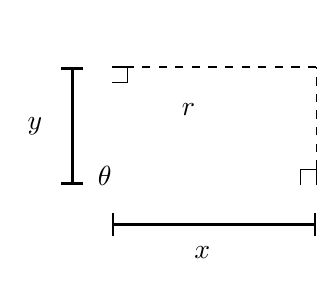
\begin{tikzpicture}[inner sep=0pt,minimum size=0mm]
\node () at (0,2){};
\node () at (1.325,-0.85) {$x$};
\node () at (-0.8,0.75) {$y$};

\node () at (40:1.5) {$r$};

\LANGLE{0,0}{3}{0}{30}{$\theta$}
\AXES{0}{0}{3}{1.7}

\draw[|-|,line width=1pt] (-0.5,0) -- (-0.5,1.5);
\draw[|-|,line width=1pt] (0,-0.5) -- (1.5*1.732,-0.5);
\draw[dashed] (1.5*1.732,1.5) -- (0,1.5);
\draw (0,1.5-0.2) -- (0.2,1.5-0.2) -- (0.2,1.5) -- (0,1.5);
\draw[dashed] (1.5*1.732,0) -- (1.5*1.732,1.5);
\draw (1.5*1.732-0.2,0) -- (1.5*1.732-0.2,0.2) -- (1.5*1.732,0.2) -- (1.5*1.732,0.0);

\end{tikzpicture}
\end{figure}

\tab$sin(\theta) = \frac{y}{r}$ \tab$cos(\theta) = \frac{x}{r}$ \tab$tan(\theta) = \frac{y}{x}$\\


\item{{\bf What is the definition of tangent?  of secant?  of cosecant?  of cotangent?}\\
{Tangent is the ratio of sine to coisine.  Secant is the reciprocal of cosine.  Cosecant is the reciprocal of sine.  Cotangent is the reciprocal of tangent.}}

\item{{\bf Is secant the reciprocal of sine or cosine?  Don't forget this!}\\
{Secant is the reciprocal of cosine.}}

\item{{\bf Why can you also use a right triangle to define sine and cosine?}\\
{If the right triangle is aligned to the x and y axes, then the projections of the hypotenuse of the triangle are equal in magnitude to the other two lines.  This can be shown using parallel lines.}}

\item{{\bf Draw a right triangle, and write the length of the sides in terms of one angle and the length of the hypotenuse.}\\
{}}

\begin{figure}[htb!]
\center
\label{fig:projection_onto_axes}
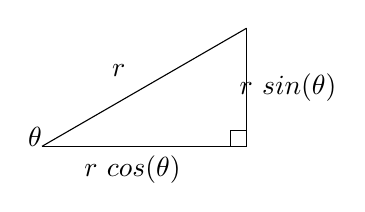
\begin{tikzpicture}[inner sep=0pt,minimum size=0mm]
\node () at (0,1.5){};
\node () at (1.325,-0.3) {$r \ cos(\theta)$};
\node () at (3.3,0.75) {$r \ sin(\theta)$};

\node () at (40:1.5) {$r$};

\LANGLE{0,0}{1}{0}{30}{$\theta$}


\draw (0,0) -- (30:3);
\draw (0,0) -- (3*0.866,0);
\draw (3*0.866,0) -- (3*0.866,3*0.5);

\draw (1.5*1.732-0.2,0) -- (1.5*1.732-0.2,0.2) -- (1.5*1.732,0.2) -- (1.5*1.732,0.0);

\end{tikzpicture}
\end{figure}

\item{{\bf From the previous question, how do you know which side corresponds with sine, and which with cosine?}\\
{The leg of the triangle opposite the angle corresponds with sine, and the leg of the triangle adjacent to the angle corresponds with cosine.}}

\end{enumerate}







\clearpage
\subsection{Chapter 4}

{\bf Practice drawing this chart, and filling in the angles.  For every angle, write the value in degrees, in radians, and the sine, cosine, and tangent.  You should be able to draw and fill out the entire chart in under five minutes.}\\

\begin{figure}[htb]
\center
\caption{Simple angles in degrees.}
\label{fig:review of simple angles}
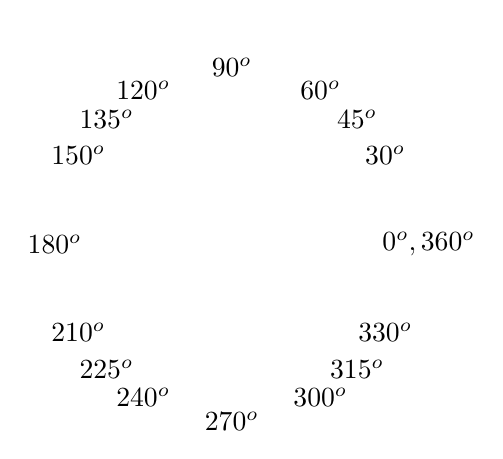
\begin{tikzpicture}[inner sep=0pt,minimum size=0mm]

\node at (0,2.75) {};

\node at (0:2.5) {$0^o, 360^o$};
\node at (30:2.25) {$30^o$};
\node at (45:2.25) {$45^o$};
\node at (60:2.25) {$60^o$};

\node at (90:2.25) {$90^o$};
\node at (120:2.25) {$120^o$};
\node at (135:2.25) {$135^o$};
\node at (150:2.25) {$150^o$};

\node at (180:2.25) {$180^o$};
\node at (210:2.25) {$210^o$};
\node at (225:2.25) {$225^o$};
\node at (240:2.25) {$240^o$};

\node at (270:2.25) {$270^o$};
\node at (300:2.25) {$300^o$};
\node at (315:2.25) {$315^o$};
\node at (330:2.25) {$330^o$};

\LLANGLE{0,0}{1.75}{0}{30}{}{0.5}
\LLANGLE{0,0}{1.75}{30}{45}{}{0.5}
\LLANGLE{0,0}{1.75}{45}{60}{}{0.5}
\LLANGLE{0,0}{1.75}{60}{90}{}{0.5}

\LLANGLE{0,0}{1.75}{90}{120}{}{0.5}
\LLANGLE{0,0}{1.75}{120}{135}{}{0.5}
\LLANGLE{0,0}{1.75}{135}{150}{}{0.5}
\LLANGLE{0,0}{1.75}{150}{180}{}{0.5}

\LLANGLE{0,0}{1.75}{180}{210}{}{0.5}
\LLANGLE{0,0}{1.75}{210}{225}{}{0.5}
\LLANGLE{0,0}{1.75}{225}{240}{}{0.5}
\LLANGLE{0,0}{1.75}{240}{270}{}{0.5}

\LLANGLE{0,0}{1.75}{270}{300}{}{0.5}
\LLANGLE{0,0}{1.75}{300}{315}{}{0.5}
\LLANGLE{0,0}{1.75}{315}{330}{}{0.5}
\LLANGLE{0,0}{1.75}{330}{360}{}{.5}

\end{tikzpicture}
\end{figure}

\begin{figure}[htb]
\center
\caption{Simple angles in radians.}
\label{fig:review of simple angles}
\begin{tikzpicture}[inner sep=0pt,minimum size=0mm]

\node at (0,2.75) {};

\node at (0:2.5) {$0^c, 2\pi^c$};
\node at (30:2.25) {$\pisix^c$};
\node at (45:2.25) {$\pifour^c$};
\node at (60:2.25) {$\pithree^c$};

\node at (90:2.25) {$\pitwo^c$};
\node at (120:2.25) {$\twopithree^c$};
\node at (135:2.25) {$\threepifour^c$};
\node at (150:2.25) {$\fivepisix^c$};

\node at (180:2.25) {$\pi^c$};
\node at (210:2.25) {$\sevenpisix^c$};
\node at (225:2.25) {$\fivepifour^c$};
\node at (240:2.25) {$\fourpithree^c$};

\node at (270:2.25) {$\threepitwo^c$};
\node at (300:2.25) {$\fivepithree^c$};
\node at (315:2.25) {$\sevenpifour^c$};
\node at (330:2.25) {$\elevenpisix^c$};

\LLANGLE{0,0}{1.75}{0}{30}{}{0.5}
\LLANGLE{0,0}{1.75}{30}{45}{}{0.5}
\LLANGLE{0,0}{1.75}{45}{60}{}{0.5}
\LLANGLE{0,0}{1.75}{60}{90}{}{0.5}

\LLANGLE{0,0}{1.75}{90}{120}{}{0.5}
\LLANGLE{0,0}{1.75}{120}{135}{}{0.5}
\LLANGLE{0,0}{1.75}{135}{150}{}{0.5}
\LLANGLE{0,0}{1.75}{150}{180}{}{0.5}

\LLANGLE{0,0}{1.75}{180}{210}{}{0.5}
\LLANGLE{0,0}{1.75}{210}{225}{}{0.5}
\LLANGLE{0,0}{1.75}{225}{240}{}{0.5}
\LLANGLE{0,0}{1.75}{240}{270}{}{0.5}

\LLANGLE{0,0}{1.75}{270}{300}{}{0.5}
\LLANGLE{0,0}{1.75}{300}{315}{}{0.5}
\LLANGLE{0,0}{1.75}{315}{330}{}{0.5}
\LLANGLE{0,0}{1.75}{330}{360}{}{.5}

\end{tikzpicture}
\end{figure}

\begin{figure}[htb]
\center
\caption{Sine of simple angles.}
\label{fig:review of simple angles}
\begin{tikzpicture}[inner sep=0pt,minimum size=0mm]

\node at (0,2.5) {};

\node at (0:2.25) {$0$};
\node at (30:2.25) {$\frac{1}{2}$};
\node at (45:2.25) {$\frac{\sqrt{2}}{2}$};
\node at (60:2.25) {$\frac{\sqrt{3}}{2}$};

\node at (90:2.25) {$1$};
\node at (120:2.25) {$\frac{\sqrt{3}}{2}$};
\node at (135:2.25) {$\frac{\sqrt{2}}{2}$};
\node at (150:2.25) {$\frac{1}{2}$};

\node at (180:2.25) {$0$};
\node at (210:2.25) {$-\frac{1}{2}$};
\node at (225:2.25) {$-\frac{\sqrt{2}}{2}$};
\node at (240:2.25) {$-\frac{\sqrt{3}}{2}$};

\node at (270:2.25) {$-1$};
\node at (300:2.25) {$-\frac{\sqrt{3}}{2}$};
\node at (315:2.25) {$-\frac{\sqrt{2}}{2}$};
\node at (330:2.25) {$-\frac{1}{2}$};

\LLANGLE{0,0}{1.75}{0}{30}{}{0.5}
\LLANGLE{0,0}{1.75}{30}{45}{}{0.5}
\LLANGLE{0,0}{1.75}{45}{60}{}{0.5}
\LLANGLE{0,0}{1.75}{60}{90}{}{0.5}

\LLANGLE{0,0}{1.75}{90}{120}{}{0.5}
\LLANGLE{0,0}{1.75}{120}{135}{}{0.5}
\LLANGLE{0,0}{1.75}{135}{150}{}{0.5}
\LLANGLE{0,0}{1.75}{150}{180}{}{0.5}

\LLANGLE{0,0}{1.75}{180}{210}{}{0.5}
\LLANGLE{0,0}{1.75}{210}{225}{}{0.5}
\LLANGLE{0,0}{1.75}{225}{240}{}{0.5}
\LLANGLE{0,0}{1.75}{240}{270}{}{0.5}

\LLANGLE{0,0}{1.75}{270}{300}{}{0.5}
\LLANGLE{0,0}{1.75}{300}{315}{}{0.5}
\LLANGLE{0,0}{1.75}{315}{330}{}{0.5}
\LLANGLE{0,0}{1.75}{330}{360}{}{.5}

\end{tikzpicture}
\end{figure}

\begin{figure}[htb]
\center
\caption{Cosine of simple angles.}
\label{fig:review of simple angles}
\begin{tikzpicture}[inner sep=0pt,minimum size=0mm]

\node at (0,2.5) {};

\node at (0:2.25) {$1$};
\node at (30:2.25) {$\frac{\sqrt{3}}{2}$};
\node at (45:2.25) {$\frac{\sqrt{2}}{2}$};
\node at (60:2.25) {$\frac{1}{2}$};

\node at (90:2.25){$0$};
\node at (120:2.25) {$-\frac{1}{2}$};
\node at (135:2.25) {$-\frac{\sqrt{2}}{2}$};
\node at (150:2.25) {$-\frac{\sqrt{3}}{2}$};

\node at (180:2.25) {$-1$};
\node at (210:2.25) {$-\frac{\sqrt{3}}{2}$};
\node at (225:2.25) {$-\frac{\sqrt{2}}{2}$};
\node at (240:2.25) {$-\frac{1}{2}$};

\node at (270:2.25) {$0$};
\node at (300:2.25) {$\frac{1}{2}$};
\node at (315:2.25) {$\frac{\sqrt{2}}{2}$};
\node at (330:2.25) {$\frac{\sqrt{3}}{2}$};

\LLANGLE{0,0}{1.75}{0}{30}{}{0.5}
\LLANGLE{0,0}{1.75}{30}{45}{}{0.5}
\LLANGLE{0,0}{1.75}{45}{60}{}{0.5}
\LLANGLE{0,0}{1.75}{60}{90}{}{0.5}

\LLANGLE{0,0}{1.75}{90}{120}{}{0.5}
\LLANGLE{0,0}{1.75}{120}{135}{}{0.5}
\LLANGLE{0,0}{1.75}{135}{150}{}{0.5}
\LLANGLE{0,0}{1.75}{150}{180}{}{0.5}

\LLANGLE{0,0}{1.75}{180}{210}{}{0.5}
\LLANGLE{0,0}{1.75}{210}{225}{}{0.5}
\LLANGLE{0,0}{1.75}{225}{240}{}{0.5}
\LLANGLE{0,0}{1.75}{240}{270}{}{0.5}

\LLANGLE{0,0}{1.75}{270}{300}{}{0.5}
\LLANGLE{0,0}{1.75}{300}{315}{}{0.5}
\LLANGLE{0,0}{1.75}{315}{330}{}{0.5}
\LLANGLE{0,0}{1.75}{330}{360}{}{.5}

\end{tikzpicture}
\end{figure}

\begin{figure}[htb]
\center
\caption{Tangent of simple angles.}
\label{fig:review of simple angles}
\begin{tikzpicture}[inner sep=0pt,minimum size=0mm]

\node at (0,2.5) {};

\node at (0:2.25) {$0$};
\node at (30:2.25) {$\frac{1}{\sqrt{3}}$};
\node at (45:2.25) {$1$};
\node at (60:2.25) {$\sqrt{3}$};

\node at (90:2.25) {$nan$};
\node at (120:2.25) {$-\sqrt{3}$};
\node at (135:2.25) {$-1$};
\node at (150:2.25) {$-\frac{1}{\sqrt{3}}$};

\node at (180:2.25) {$0$};
\node at (210:2.25) {$\frac{1}{\sqrt{3}}$};
\node at (225:2.25) {$1$};
\node at (240:2.25) {$\sqrt{3}$};

\node at (270:2.25) {$nan$};
\node at (300:2.25) {$-\sqrt{3}$};
\node at (315:2.25) {$-1$};
\node at (330:2.25) {$-\frac{1}{\sqrt{3}}$};

\LLANGLE{0,0}{1.75}{0}{30}{}{0.5}
\LLANGLE{0,0}{1.75}{30}{45}{}{0.5}
\LLANGLE{0,0}{1.75}{45}{60}{}{0.5}
\LLANGLE{0,0}{1.75}{60}{90}{}{0.5}

\LLANGLE{0,0}{1.75}{90}{120}{}{0.5}
\LLANGLE{0,0}{1.75}{120}{135}{}{0.5}
\LLANGLE{0,0}{1.75}{135}{150}{}{0.5}
\LLANGLE{0,0}{1.75}{150}{180}{}{0.5}

\LLANGLE{0,0}{1.75}{180}{210}{}{0.5}
\LLANGLE{0,0}{1.75}{210}{225}{}{0.5}
\LLANGLE{0,0}{1.75}{225}{240}{}{0.5}
\LLANGLE{0,0}{1.75}{240}{270}{}{0.5}

\LLANGLE{0,0}{1.75}{270}{300}{}{0.5}
\LLANGLE{0,0}{1.75}{300}{315}{}{0.5}
\LLANGLE{0,0}{1.75}{315}{330}{}{0.5}
\LLANGLE{0,0}{1.75}{330}{360}{}{.5}

\end{tikzpicture}
\end{figure}









\clearpage
\subsection{Chapter 5}

{\bf Draw and label graphs for the six trig. functions: sine, cosine, tangent, secant, cosecant, and cotangent.  You should be able to draw all of these from memory, without referring back to the text.}\\

\begin{figure}[htb]
\center
\caption{Graph of sine.}
\label{fig:graph of sine}
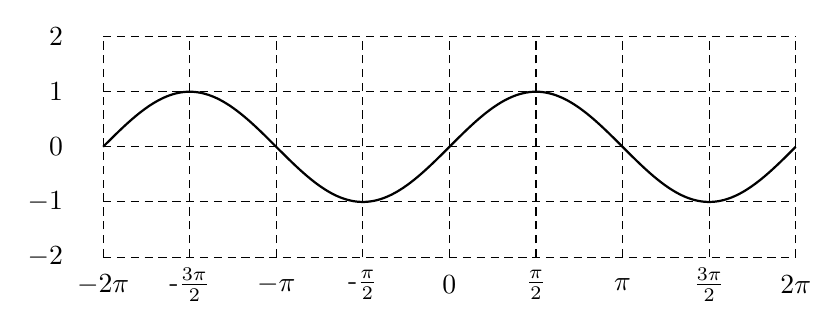
\begin{tikzpicture}[inner sep=0pt,minimum size=0mm, scale = 0.7]

\node at (3.1415, -2.5) {$\pi$};
\node at (3/2*3.1415, -2.5) {$\frac{3\pi}{2}$};
\node at (2*3.1415, -2.5) {$2\pi$};
\node at (1/2*3.1415, -2.5) {$\frac{\pi}{2}$};
\node at (0, -2.5) {$0$};
\node at (1/2*-3.1415, -2.5) {-$\frac{\pi}{2}$};
\node at (-3.1415, -2.5) {$-\pi$};
\node at (3/2*-3.1415, -2.5) {-$\frac{3\pi}{2}$};
\node at (2*-3.1415, -2.5) {$-2\pi$};

\node[left] at (-7,2) {$2$};
\node[left] at (-7,1) {$1$};
\node[left] at (-7,0) {$0$};
\node[left] at (-7,-1) {$-1$};
\node[left] at (-7,-2) {$-2$};

\draw[xstep=3.1415/2, densely dashed] (-2*3.1415,-2) grid (2*3.1415,2);
\AXES{0}{0}{2*3.1415}{2}
\draw[thick, variable = \t, domain=2*-3.1415:2*3.1415,samples=250] plot ({\t},{sin(180*\t/3.1415)});

\end{tikzpicture}
\end{figure}


\begin{figure}[htb]
\center
\caption{Graph of cosine.}
\label{fig:graph of cosine}
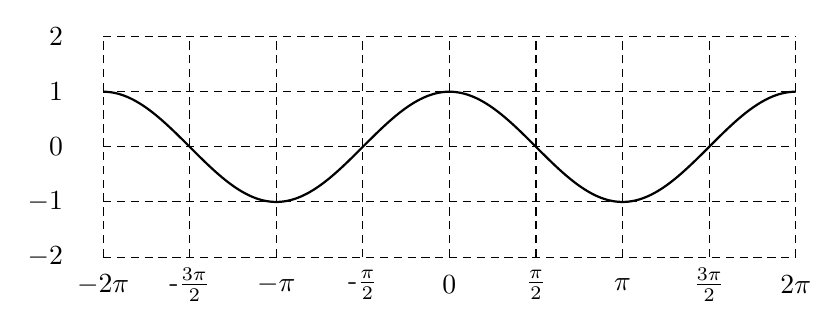
\begin{tikzpicture}[inner sep=0pt,minimum size=0mm, scale = 0.7]

\node at (3.1415, -2.5) {$\pi$};
\node at (3/2*3.1415, -2.5) {$\frac{3\pi}{2}$};
\node at (2*3.1415, -2.5) {$2\pi$};
\node at (1/2*3.1415, -2.5) {$\frac{\pi}{2}$};
\node at (0, -2.5) {$0$};
\node at (1/2*-3.1415, -2.5) {-$\frac{\pi}{2}$};
\node at (-3.1415, -2.5) {$-\pi$};
\node at (3/2*-3.1415, -2.5) {-$\frac{3\pi}{2}$};
\node at (2*-3.1415, -2.5) {$-2\pi$};

\node[left] at (-7,2) {$2$};
\node[left] at (-7,1) {$1$};
\node[left] at (-7,0) {$0$};
\node[left] at (-7,-1) {$-1$};
\node[left] at (-7,-2) {$-2$};

\draw[xstep=3.1415/2, densely dashed] (-2*3.1415,-2) grid (2*3.1415,2);
\AXES{0}{0}{2*3.1415}{2}
\draw[thick, variable = \t, domain=2*-3.1415:2*3.1415,samples=250] plot ({\t},{cos(180*\t/3.1415)});

\end{tikzpicture}
\end{figure}


\begin{figure}[htb]
\center
\caption{Graph of tangent.}
\label{fig:graph of tan}
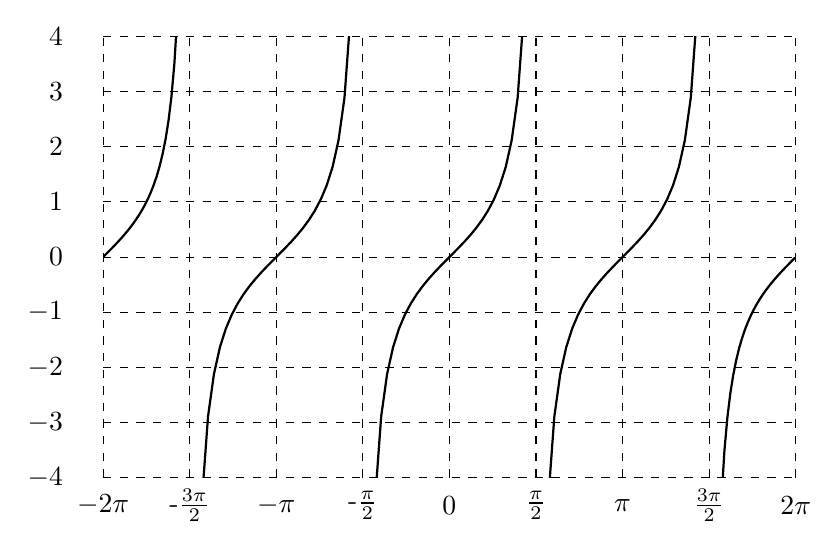
\begin{tikzpicture}[inner sep=0pt,minimum size=0mm, scale = 0.7]

\node at (3.1415, -4.5) {$\pi$};
\node at (3/2*3.1415, -4.5) {$\frac{3\pi}{2}$};
\node at (2*3.1415, -4.5) {$2\pi$};
\node at (1/2*3.1415, -4.5) {$\frac{\pi}{2}$};
\node at (0, -4.5) {$0$};
\node at (1/2*-3.1415, -4.5) {-$\frac{\pi}{2}$};
\node at (-3.1415, -4.5) {$-\pi$};
\node at (3/2*-3.1415, -4.5) {-$\frac{3\pi}{2}$};
\node at (2*-3.1415, -4.5) {$-2\pi$};

\node[left] at (-7,4) {$4$};
\node[left] at (-7,3) {$3$};
\node[left] at (-7,2) {$2$};
\node[left] at (-7,1) {$1$};
\node[left] at (-7,0) {$0$};
\node[left] at (-7,-1) {$-1$};
\node[left] at (-7,-2) {$-2$};
\node[left] at (-7,-3) {$-3$};
\node[left] at (-7,-4) {$-4$};

\draw[xstep=3.1415/2, dashed] (-2*3.1415,-4) grid (2*3.1415,4);
\AXES{0}{0}{2*3.1415}{4}

\begin{scope}
    \clip(2*-3.1415,-4) rectangle (2*3.1415,4);

\draw[thick,
 variable = \t, 
 domain=4/2*-3.1415+0.01:3/2*-3.1415-0.01,
 samples=30] 
plot ({\t},{tan(180*\t/3.1415)});


\draw[thick,
 variable = \t, 
 domain=3/2*-3.1415+0.01:1/2*-3.1415-0.01,
 samples=30] 
plot ({\t},{tan(180*\t/3.1415)});

\draw[thick,
 variable = \t, 
 domain=1/2*-3.1415+0.01:1/2*3.1415-0.01,
 samples=30] 
plot ({\t},{tan(180*\t/3.1415)});

\draw[thick,
 variable = \t, 
 domain=1/2*3.1415+0.01:3/2*3.1415-0.01,
 samples=30] 
plot ({\t},{tan(180*\t/3.1415)});

\draw[thick,
 variable = \t, 
 domain=3/2*3.1415+0.01:4/2*3.1415-0.01,
 samples=30] 
plot ({\t},{tan(180*\t/3.1415)});

\end{scope}

\end{tikzpicture}
\end{figure}



\begin{figure}[htb]
\center
\caption{Graph of secant.}
\label{fig:graph of sec}
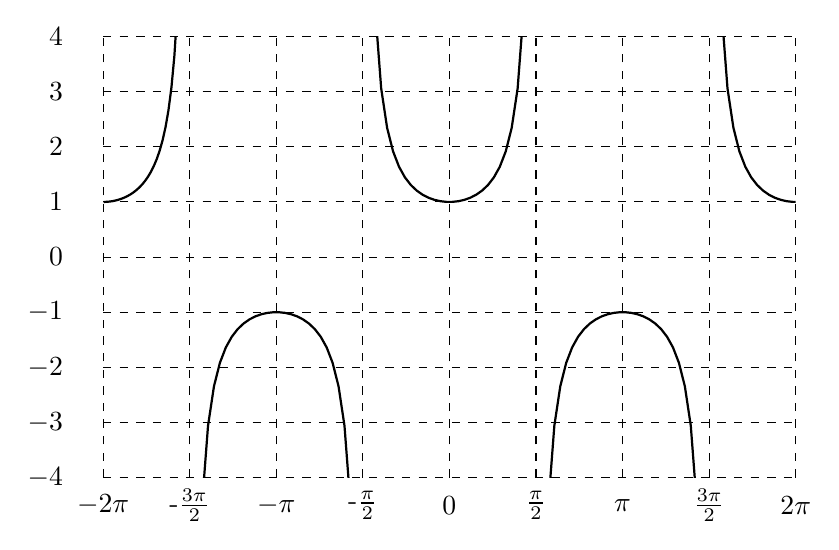
\begin{tikzpicture}[inner sep=0pt,minimum size=0mm, scale = 0.7]

\node at (3.1415, -4.5) {$\pi$};
\node at (3/2*3.1415, -4.5) {$\frac{3\pi}{2}$};
\node at (2*3.1415, -4.5) {$2\pi$};
\node at (1/2*3.1415, -4.5) {$\frac{\pi}{2}$};
\node at (0, -4.5) {$0$};
\node at (1/2*-3.1415, -4.5) {-$\frac{\pi}{2}$};
\node at (-3.1415, -4.5) {$-\pi$};
\node at (3/2*-3.1415, -4.5) {-$\frac{3\pi}{2}$};
\node at (2*-3.1415, -4.5) {$-2\pi$};

\node[left] at (-7,4) {$4$};
\node[left] at (-7,3) {$3$};
\node[left] at (-7,2) {$2$};
\node[left] at (-7,1) {$1$};
\node[left] at (-7,0) {$0$};
\node[left] at (-7,-1) {$-1$};
\node[left] at (-7,-2) {$-2$};
\node[left] at (-7,-3) {$-3$};
\node[left] at (-7,-4) {$-4$};

\draw[xstep=3.1415/2, dashed] (-2*3.1415,-4) grid (2*3.1415,4);
\AXES{0}{0}{2*3.1415}{4}

\begin{scope}
    \clip(2*-3.1415,-4) rectangle (2*3.1415,4);

\draw[thick,
 variable = \t, 
 domain=4/2*-3.1415+0.01:3/2*-3.1415-0.01,
 samples=30] 
plot ({\t},{1/cos(180*\t/3.1415)});

\draw[thick,
 variable = \t, 
 domain=3/2*-3.1415+0.01:1/2*-3.1415-0.01,
 samples=30] 
plot ({\t},{1/cos(180*\t/3.1415)});

\draw[thick,
 variable = \t, 
 domain=1/2*-3.1415+0.01:1/2*3.1415-0.01,
 samples=30] 
plot ({\t},{1/cos(180*\t/3.1415)});

\draw[thick,
 variable = \t, 
 domain=1/2*3.1415+0.01:3/2*3.1415-0.01,
 samples=30] 
plot ({\t},{1/cos(180*\t/3.1415)});

\draw[thick,
 variable = \t, 
 domain=3/2*3.1415+0.01:5/2*3.1415-0.01,
 samples=30] 
plot ({\t},{1/cos(180*\t/3.1415)});

\end{scope}

\end{tikzpicture}
\end{figure}


\begin{figure}[htb]
\center
\caption{Graph of cosecant.}
\label{fig:graph of csc}
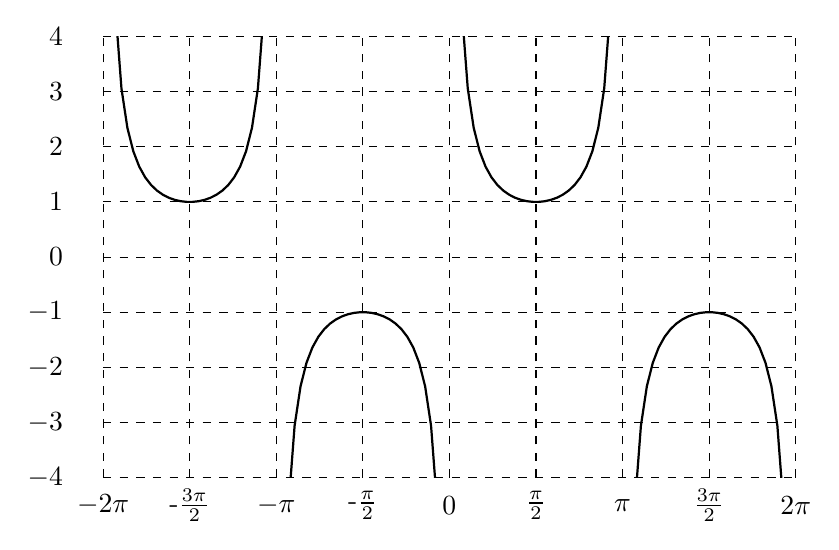
\begin{tikzpicture}[inner sep=0pt,minimum size=0mm, scale = 0.7]

\node at (3.1415, -4.5) {$\pi$};
\node at (3/2*3.1415, -4.5) {$\frac{3\pi}{2}$};
\node at (2*3.1415, -4.5) {$2\pi$};
\node at (1/2*3.1415, -4.5) {$\frac{\pi}{2}$};
\node at (0, -4.5) {$0$};
\node at (1/2*-3.1415, -4.5) {-$\frac{\pi}{2}$};
\node at (-3.1415, -4.5) {$-\pi$};
\node at (3/2*-3.1415, -4.5) {-$\frac{3\pi}{2}$};
\node at (2*-3.1415, -4.5) {$-2\pi$};

\node[left] at (-7,4) {$4$};
\node[left] at (-7,3) {$3$};
\node[left] at (-7,2) {$2$};
\node[left] at (-7,1) {$1$};
\node[left] at (-7,0) {$0$};
\node[left] at (-7,-1) {$-1$};
\node[left] at (-7,-2) {$-2$};
\node[left] at (-7,-3) {$-3$};
\node[left] at (-7,-4) {$-4$};

\draw[xstep=3.1415/2, dashed] (-2*3.1415,-4) grid (2*3.1415,4);
\AXES{0}{0}{2*3.1415}{4}

\begin{scope}
    \clip(2*-3.1415,-4) rectangle (2*3.1415,4);

\draw[thick,
 variable = \t, 
 domain=4/2*-3.1415+0.01:2/2*-3.1415-0.01,
 samples=30] 
plot ({\t},{1/sin(180*\t/3.1415)});

\draw[thick,
 variable = \t, 
 domain=2/2*-3.1415+0.01:0/2*-3.1415-0.01,
 samples=30] 
plot ({\t},{1/sin(180*\t/3.1415)});

\draw[thick,
 variable = \t, 
 domain=0/2*-3.1415+0.01:2/2*3.1415-0.01,
 samples=30] 
plot ({\t},{1/sin(180*\t/3.1415)});

\draw[thick,
 variable = \t, 
 domain=2/2*3.1415+0.01:4/2*3.1415-0.01,
 samples=30] 
plot ({\t},{1/sin(180*\t/3.1415)});

\end{scope}

\end{tikzpicture}
\end{figure}


\begin{figure}[htb]
\center
\caption{Graph of cotangent.}
\label{fig:graph of cot}
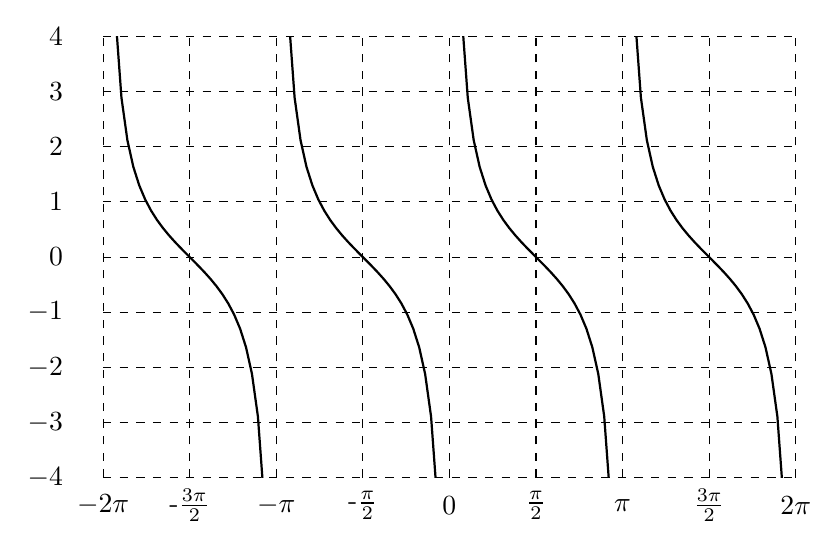
\begin{tikzpicture}[inner sep=0pt,minimum size=0mm, scale = 0.7]

\node at (3.1415, -4.5) {$\pi$};
\node at (3/2*3.1415, -4.5) {$\frac{3\pi}{2}$};
\node at (2*3.1415, -4.5) {$2\pi$};
\node at (1/2*3.1415, -4.5) {$\frac{\pi}{2}$};
\node at (0, -4.5) {$0$};
\node at (1/2*-3.1415, -4.5) {-$\frac{\pi}{2}$};
\node at (-3.1415, -4.5) {$-\pi$};
\node at (3/2*-3.1415, -4.5) {-$\frac{3\pi}{2}$};
\node at (2*-3.1415, -4.5) {$-2\pi$};

\node[left] at (-7,4) {$4$};
\node[left] at (-7,3) {$3$};
\node[left] at (-7,2) {$2$};
\node[left] at (-7,1) {$1$};
\node[left] at (-7,0) {$0$};
\node[left] at (-7,-1) {$-1$};
\node[left] at (-7,-2) {$-2$};
\node[left] at (-7,-3) {$-3$};
\node[left] at (-7,-4) {$-4$};

\draw[xstep=3.1415/2, dashed] (-2*3.1415,-4) grid (2*3.1415,4);
\AXES{0}{0}{2*3.1415}{4}

\begin{scope}
    \clip(2*-3.1415,-4) rectangle (2*3.1415,4);

\draw[thick,
 variable = \t, 
 domain=4/2*-3.1415+0.01:2/2*-3.1415-0.01,
 samples=30] 
plot ({\t},{1/tan(180*\t/3.1415)});

\draw[thick,
 variable = \t, 
 domain=2/2*-3.1415+0.01:0/2*-3.1415-0.01,
 samples=30] 
plot ({\t},{1/tan(180*\t/3.1415)});

\draw[thick,
 variable = \t, 
 domain=0/2*-3.1415+0.01:2/2*3.1415-0.01,
 samples=30] 
plot ({\t},{1/tan(180*\t/3.1415)});

\draw[thick,
 variable = \t, 
 domain=2/2*3.1415+0.01:4/2*3.1415-0.01,
 samples=30] 
plot ({\t},{1/tan(180*\t/3.1415)});
\end{scope}

\end{tikzpicture}
\end{figure}









\clearpage
\subsection{Chapter 6}

\begin{enumerate}

\item{{\bf Find 3 equivalent angles for each of the following:}\\

\tab a) $30^o \simeq  ..., -690^o, -330^o, 390^o, 750^o, ...$\\

\tab b) $\frac{7\pi}{6}^c \simeq ..., \frac{-17\pi}{6}^c, \frac{-5\pi}{6}^c, \frac{19\pi}{6}^c, \frac{31\pi}{6}^c, ...$\\

\tab c) $115^o \simeq  ..., -605^o, -245^o, 475^o, 835^o, ...$\\

\tab d) $\frac{-\pi}{2}^c \simeq ..., \frac{-9\pi}{2}^c, \frac{-5\pi}{2}^c, \frac{3\pi}{2}^c, \frac{7\pi}{2}^c, ...$\\

\tab e) $0^o  \simeq  ..., -720^o, -360^o, 360^o, 720^o, ...$\\}

\item{{\bf Write whether each of the following trig. functions are even, odd, or neither, and prove it:}\\

\tab a) $tan(\theta)$\\

\tab\tab $tan(\theta) = \frac{sin(\theta)}{cos(\theta)}$\\

\tab\tab$\implies tan(-\theta) = \frac{sin(-\theta)}{cos(-\theta)}$\\

\tab\tab $sin(-\theta) = - sin(\theta)$ and $cos(-\theta)=cos(\theta)$\\

\tab\tab$\implies \frac{sin(-\theta)}{cos(-\theta)}  = \frac{-sin(\theta)}{cos(\theta)} = -tan(\theta)$\\

\tab\tab $\implies tan(-\theta) = - tan(\theta)$\\

\tab\tab Tangent is {\bf odd}.\\

\tab b) $cot(\theta)$\\

\tab\tab $cot(-\theta) = \frac{1}/{tan(-\theta)}$\\

\tab\tab $= - \frac{1}{tan(\theta)}$\\

\tab\tab $= -cot(\theta)$\\

\tab\tab Cotangent is {\bf even}.\\

\tab c) $sec(\theta)$\\

\tab\tab $sec(-\theta) = \frac{1}{cos(-\theta)}$\\

\tab\tab $= \frac{1}{cos(\theta)} = sec(\theta)$\\

\tab\tab Secant is {\bf even}.\\

\tab d) $csc(\theta)$\\

\tab\tab $csc(-theta) = \frac{1}{sin(-\theta)}$\\

\tab\tab $= \frac{1}{-sin(\theta)} = - csc(theta)$\\

\tab\tab Cosecant is {\bf odd}.\\

\tab e) $sin(\theta) - cos(\theta)$\\}

\tab\tab $sin(-\theta) - cos(-\theta) = -sin(\theta) - cos(\theta)$\\

\tab\tab $-sin(\theta) - cos(\theta) \neq sin(\theta) - cos(\theta)$\\

\tab\tab $sin(\theta) - cos(\theta)$ is {\bf neither}.\\	

\item{Simplify the following expressions:\\

\tab a) $cos^2(\theta)tan(\theta)$\\

\tab\tab $cos^2(\theta)tan(\theta) = cos^2(\theta)\frac{sin(\theta)}{cos(\theta)}$\\

\tab\tab $= sin(\theta)cos(\theta)$\\

\tab b) $csc(\theta) - cos(\theta)cot(\theta)$\\

\tab\tab $csc(\theta) - cos(\theta)cot(\theta)$\\

\tab\tab $= \frac{1}{sin(\theta)} - cos(\theta)\frac{cos(\theta)}{sin(\theta)}$\\

\tab\tab $= \frac{1}{sin(\theta)} - \frac{cos^2(\theta)}{sin(\theta)}$\\

\tab\tab $= \frac{1 - cos^2(\theta)}{sin(\theta)}$\\

\tab\tab $= \frac{sin^2(\theta)}{sin(\theta)}$\\

\tab\tab $= sin(\theta)$\\

\tab c) $1 + cot^2(\theta)$\\

\tab\tab $1 + cot^2(\theta)$\\

\tab\tab $= 1 + \frac{cos^2(\theta)}{sin^2(\theta)}$\\

\tab\tab $= \frac{sin^2(\theta)}{sin^2(\theta)} + \frac{cos^2(\theta)}{sin^2(\theta)}$\\

\tab\tab $= \frac{sin^2(\theta) + cos^2(\theta)}{sin^2(\theta)}$\\

\tab\tab $= \frac{1}{sin^2(\theta)}$\\

\tab\tab $= csc^2(\theta)$\\

\tab d) $\frac{sin^2(\theta)tan^2(\theta) + sin^2(\theta)}{tan^2(\theta)}$\\

\tab\tab $\frac{sin^2(\theta)tan^2(\theta) + sin^2(\theta)}{tan^2(\theta)}$\\

\tab\tab $= \frac{sin^2(\theta)tan^2(\theta) + sin^2(\theta)}{tan^2(\theta)}$\\

\tab\tab $= \frac{sin^2(\theta)tan^2(\theta)}{tan^2(\theta)} + \frac{sin^2(\theta)}{tan^2(\theta)}$\\

\tab\tab $= sin^2(\theta) + sin^2(\theta)cot^2(\theta)$\\

\tab\tab $= sin^2(\theta) + sin^2(\theta)\frac{cos^2(\theta)}{sin^2(\theta)}$\\

\tab\tab $= sin^2(\theta) + cos^2(\theta)$\\

\tab\tab $= 1$\\

\tab e) $\frac{(sec(\theta) + tan(\theta))(sec(\theta) - tan(\theta))}{(csc(\theta) - cot(\theta))(csc(\theta) + cot(\theta))}$\\}

\tab\tab $\frac{(sec(\theta) + tan(\theta))(sec(\theta) - tan(\theta))}{(csc(\theta) - cot(\theta))(csc(\theta) + cot(\theta))}$\\

\tab\tab $= \frac{sec^2(\theta) - tan^2(\theta)}{csc^2(\theta) - cot^2(\theta)}$\\

\tab\tab $= \frac{1}{1}$\\

\tab\tab $= 1$\\

\item{\bf Given that the sine of an angle is 0.73, what is the cosine?  the tangent?\\}

\tab $sin(\theta) = 0.73$ and $sin^2(\theta) + cos^2(\theta) = 1$\\

\tab $\implies 0.73^2 + cos^2(\theta) = 1$\\

\tab $\implies 0.5329 + cos^2(\theta) = 1$\\

\tab $\implies cos^2(\theta) = 0.4671$\\

\tab $\implies cos(\theta) = \pm 0.6834$\\

\tab $tan(\theta) = \frac{sin(\theta)}{cos(\theta)}$\\

\tab $= \frac{0.73}{\pm 0.6834}$\\

\tab $= \pm 1.0681$\\

\item{Given that the tangent of an angle is 0.5 and the angle is in the first quadrant, what is the cosine?}

\tab $tan(\theta) = 0.5$\\

\tab $\implies \frac{sin(\theta)}{cos(\theta)} = 0.5$\\

\tab $\implies sin(\theta) = 0.5cos(\theta)$\\

\tab $sin^2(\theta) + cos^2(\theta) = 1$\\

\tab $\implies (0.5cos(\theta))^2 + cos^2(\theta) = 1$\\

\tab $\implies 0.25cos^2(\theta) + cos^2(\theta) = 1$\\

\tab $\implies 1.25cos^2(\theta) = 1$\\

\tab $\implies cos^2(\theta) = \frac{1}{1.25} = \frac{4}{5}$\\

\tab $\implies cos(\theta) = \frac{2}{\sqrt{5}}$\\

\end{enumerate}












\clearpage
\subsection{Chapter 7}

\begin{enumerate}

\item{{\bf What is the definition of the inverse of a function?}\\
{The inverse of a function $f(x)$ is the function $g(x)$, where $g(f(x))=x$}\\}

\item{\bf Write the inverse of each of the following functions:}\\

\tab a) $f(x) = x + 1$\\

\tab \tab $f(x) = x + 1$\\

\tab \tab $\implies x = f^{-1}(x) + 1$\\

\tab \tab $\implies f^{-1}(x) = x - 1$\\

\tab b) $f(x) = x^2$\\

\tab \tab $f(x) = x^2$\\

\tab \tab $\implies x = (f^{-1}(x))^2$\\

\tab \tab $\implies f^{-1}(x) = \sqrt{x}$\\

\tab c) $f(x) = \frac{1}{x}$\\

\tab \tab $f(x) = \frac{1}{x}$\\

\tab \tab $\implies x = \frac{1}{f^{-1}(x)}$\\

\tab \tab $\implies f^{-1}(x) = \frac{1}{x}$\\

\tab \tab Note:  The inverse of $\frac{1}{x}$ is itself.  Any function that has reflective symmetry across the diagonal $y = x$ will be its own inverse.\\

\tab d) $f(x) = sin(x)$\\

\tab \tab $f^{-1}(x) = arcsin(x)$\\

\tab e) $f(x) = 1$\\

\tab \tab $f(x) = 1$\\

\tab \tab $\implies x = ?$\\

\tab \tab This function has no inverse.  The inverse of this function is a relation, not a function.\\

\item{{\bf What is the difference between a relation and a function?}\\
{A function is a mapping where each input value corresponds to exactly one output value.  A relation is also a mapping of inputs to outputs, but each input may map to multiple outputs.}\\}


\item{{\bf Why do inverse trig. functions have a principal-value range?}\\
{Trig functions are periodic, and as a result, the inverse of any trig function is not a function, but a relation.  So what do we do?  We cheat, and constrain each inverse trig. relation to a range of half of its period.  When we do this, there are no repeating values and we can treat them as a functions.}\\}

\item{\bf Draw and label a graph of the arc-sine, arc-cosine, and arc-tangent, without referring back to the text.}\\

\begin{figure}[htb!]
\center
\caption{Arc-sine constrained to its principal-value range.}
\label{fig:principal value arc sine}
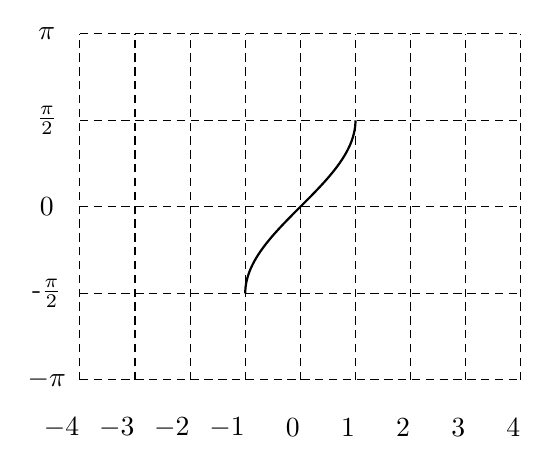
\begin{tikzpicture}[inner sep=0pt,minimum size=0mm, scale = 0.7]

\node at (-4.6,3.1415) {$\pi$};
\node at (-4.6,1/2*3.1415) {$\frac{\pi}{2}$};
\node at (-4.6,0) {$0$};
\node at (-4.6,1/2*-3.1415) {-$\frac{\pi}{2}$};
\node at (-4.6,-3.1415) {$-\pi$};

\node[left] at (4, -4) {$4$};
\node[left] at (3, -4) {$3$};
\node[left] at (2, -4) {$2$};
\node[left] at (1, -4) {$1$};
\node[left] at (0, -4) {$0$};
\node[left] at (-1, -4) {$-1$};
\node[left] at (-2, -4) {$-2$};
\node[left] at (-3, -4) {$-3$};
\node[left] at (-4, -4) {$-4$};

\draw[ystep=3.1415/2, densely dashed] (-4,-1*3.1415) grid (4,1*3.1415);
\AXES{0}{0}{4}{1*3.1415}
\draw[thick, variable = \t, domain=1/2*-3.1415:1/2*3.1415,samples=250] plot ({sin(180*\t/3.1415)},{\t});

\end{tikzpicture}
\end{figure}

\begin{figure}[htb!]
\center
\caption{Arc-cosine constrained to its principal-value range.}
\label{fig:principal value arc-cosine }
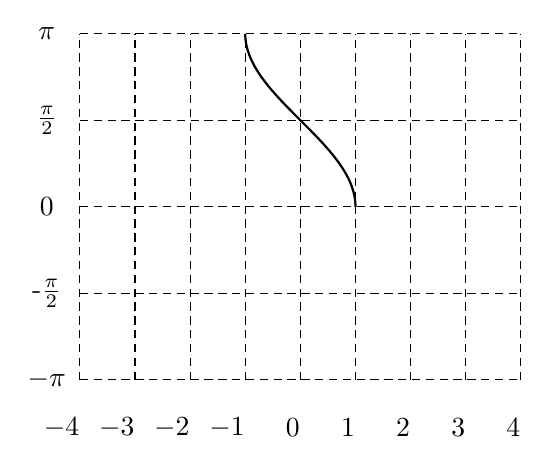
\begin{tikzpicture}[inner sep=0pt,minimum size=0mm, scale = 0.7]

\node at (-4.6,3.1415) {$\pi$};
\node at (-4.6,1/2*3.1415) {$\frac{\pi}{2}$};
\node at (-4.6,0) {$0$};
\node at (-4.6,1/2*-3.1415) {-$\frac{\pi}{2}$};
\node at (-4.6,-3.1415) {$-\pi$};

\node[left] at (4, -4) {$4$};
\node[left] at (3, -4) {$3$};
\node[left] at (2, -4) {$2$};
\node[left] at (1, -4) {$1$};
\node[left] at (0, -4) {$0$};
\node[left] at (-1, -4) {$-1$};
\node[left] at (-2, -4) {$-2$};
\node[left] at (-3, -4) {$-3$};
\node[left] at (-4, -4) {$-4$};

\draw[ystep=3.1415/2, densely dashed] (-4,-1*3.1415) grid (4,1*3.1415);
\AXES{0}{0}{4}{1*3.1415}
\draw[thick, variable = \t, domain=0:3.1415,samples=250] plot ({cos(180*\t/3.1415)},{\t});

\end{tikzpicture}
\end{figure}


\begin{figure}[htb!]
\center
\caption{Arc-tangent contrained to its principal-value range.}
\label{fig:principal value arc-tan}
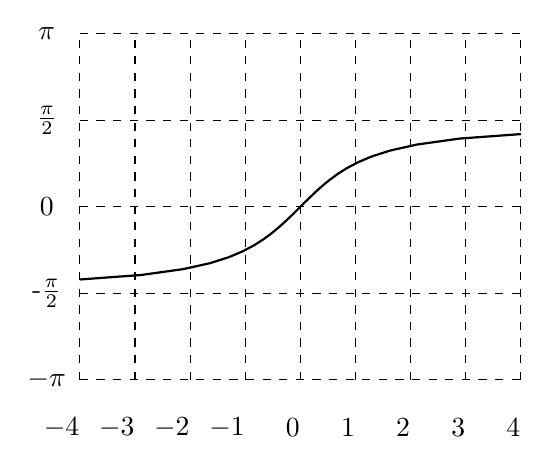
\begin{tikzpicture}[inner sep=0pt,minimum size=0mm, scale = 0.7]

\node at (-4.6, 3.1415) {$\pi$};
\node at (-4.6, 1/2*3.1415) {$\frac{\pi}{2}$};
\node at (-4.6, 0) {$0$};
\node at (-4.6, 1/2*-3.1415) {-$\frac{\pi}{2}$};
\node at (-4.6, -3.1415) {$-\pi$};

\node[left] at (4, -4) {$4$};
\node[left] at (3, -4) {$3$};
\node[left] at (2, -4) {$2$};
\node[left] at (1, -4) {$1$};
\node[left] at (0, -4) {$0$};
\node[left] at (-1, -4) {$-1$};
\node[left] at (-2, -4) {$-2$};
\node[left] at (-3, -4) {$-3$};
\node[left] at (-4, -4) {$-4$};

\draw[ystep=3.1415/2, dashed] (-4,-3.1415) grid (4,3.1415);
\AXES{0}{0}{4}{3.1415}

\begin{scope}
    \clip(-4, -3.1415) rectangle (4, 3.1415);

\draw[thick,
 variable = \t, 
 domain=1/2*-3.1415+0.01:1/2*3.1415-0.01,
 samples=30] 
plot ({tan(180*\t/3.1415)}, {\t});

\end{scope}

\end{tikzpicture}
\end{figure}



\end{enumerate}










\clearpage
\subsection{Chapter 8}

\begin{enumerate}

\item{\bf Write down the formulae for the sine, cosine, and tangent of the sum of two angles until you've committed them to memory.}\\

\tab$sin(\alpha \pm \beta) = sin(\alpha)cos(\beta) \pm cos(\alpha)sin(\beta)$\\

\tab$cos(\alpha \pm \beta) = cos(\alpha)cos(\beta) \mp sin(\alpha)sin(\beta)$\\

\tab$tan(\alpha \pm \beta) = \frac{tan(\alpha) \pm tan(\beta)}{1 \mp tan(\alpha)tan(\beta)}$\\



\item{\bf Using the previous formulae, derive the double angle formulae for sine, cosine, and tangent}\\

\tab$sin(\alpha \pm \beta) = sin(\alpha)cos(\beta) \pm cos(\alpha)sin(\beta)$\\

\tab$\implies sin(\alpha + \alpha) = sin(\alpha)cos(\alpha) + cos(\alpha)sin(\alpha)$\\

\tab$\implies sin(2\alpha) = 2sin(\alpha)cos(\alpha)$\\ \\


\tab$cos(\alpha \pm \beta) = cos(\alpha)cos(\beta) \mp sin(\alpha)sin(\beta)$\\

\tab$\implies cos(\alpha + \alpha) = cos(\alpha)cos(\alpha) - sin(\alpha)sin(\alpha)$\\

\tab$\implies cos(2\alpha) = cos^2(\alpha) - sin^2(\alpha)$\\ \\


\tab$tan(\alpha \pm \beta) = \frac{tan(\alpha) \pm tan(\beta)}{1 \mp tan(\alpha)tan(\beta)}$\\

\tab$\implies tan(\alpha + \alpha) = \frac{tan(\alpha) + tan(\alpha)}{1 - tan(\alpha)tan(\alpha)}$\\

\tab$\implies tan(2\alpha) = \frac{2tan(\alpha)}{1 - tan^2(\alpha)}$\\

\item{\bf Using the previous formulae, derive the half angle formulae for sine, cosine, and tangent}\\

Using the double angle formulae for the cosine, and the Pythagorean identitiy, we can also derive equations for the half-angle of the sine and cosine.\\

\tab$cos(2\alpha) = cos^2(\alpha) - sin^2(\alpha)$\\

\tab$\implies cos(\alpha) = cos^2(\frac{\alpha}{2}) - sin^2(\frac{\alpha}{2})$\\

\tab$\implies cos(\alpha) = (1 - sin^2(\frac{\alpha}{2})) - sin^2(\frac{\alpha}{2})$\\

\tab$\implies cos(\alpha) = 1- 2sin^2(\frac{\alpha}{2})$\\

\tab$\implies \frac{1 - cos(\alpha)}{2} = sin^2(\frac{\alpha}{2})$\\

\tab$\implies sin(\frac{\alpha}{2}) = (\frac{1 - cos(\alpha)}{2})^{\frac{1}{2}}$\\ \\



\tab$cos(2\alpha) = cos^2(\alpha) - sin^2(\alpha)$\\

\tab$\implies cos(\alpha) = cos^2(\frac{\alpha}{2}) - sin^2(\frac{\alpha}{2})$\\

\tab$\implies cos(\alpha) = cos^2(\frac{\alpha}{2}) - (1 - cos^2(\frac{\alpha}{2}))$\\

\tab$\implies cos(\alpha) = 2cos^2(\frac{\alpha}{2}) -  1$\\

\tab$\implies \frac{1 + cos(\alpha)}{2} = cos^2(\frac{\alpha}{2})$\\

\tab$\implies cos(\frac{\alpha}{2}) = (\frac{1 + cos(\alpha)}{2})^{\frac{1}{2}}$\\ \\


\tab$tan(\frac{\alpha}{2}) = \frac{sin(\frac{\alpha}{2})}{cos(\frac{\alpha}{2})}$\\

\tab$ = \frac{ (\frac{1 - cos(\alpha)}{2})^{\frac{1}{2}}}{ (\frac{1 + cos(\alpha)}{2})^{\frac{1}{2}}} = (\frac{\frac{1 - cos(\alpha)}{2}}{\frac{1 + cos(\alpha)}{2}})^{\frac{1}{2}}$\\

\tab$ = (\frac{1 - cos(\alpha)}{1 + cos(\alpha)})^{\frac{1}{2}}$\\

\end{enumerate}





\clearpage
\subsection{Chapter 9}

\begin{enumerate}

\item{\bf Write the conversions from rectangular to polar coordinates, and the conversions from polar to rectangular coordinates, until you've committed them to memory.}\\

\tab Polar to rectangular:\\

\tab$y = rsin(\theta)$ \ \ \ and \ \ \ $x = rcos(\theta)$\\ \\

\tab Rectangular to polar:\\

\tab$r = \sqrt{x^2 + y^2}$\\

\tab$\theta = arcsin(\frac{y}{r})$ \ \ or \ \ $\theta = arccos(\frac{x}{r})$ \ \ or \ \ $\theta = arctan(\frac{y}{x})$\\

\item{\bf Convert the following coordinates from polar to rectangular:}\\

\tab a) $(1,0^c)$\\

\tab \tab $x = r cos(\theta) = 1 cos(0) = 1$\\

\tab \tab $y = r sin(\theta) = 1 sin(0) = 0$\\

\tab b) $(2,\frac{\pi}{4}^c)$\\

\tab \tab $x = 2 cos(\frac{\pi}{4}) = 2 \frac{\sqrt{2}}{2} = \sqrt{2}$\\

\tab \tab $y = 2 sin(\frac{\pi}{4}) = 2 \frac{\sqrt{2}}{2} = \sqrt{2}$\\

\tab c) $(1,115^o)$\\

\tab \tab $x = 1 cos(115^o) = -0.4226$\\

\tab \tab $y = 1 sin(115^o) = 0.9063$\\

\tab d) $(2,-30^o)$\\

\tab \tab $x = 2 cos(-30^o) = 2 \frac{\sqrt{3}}{2} = \sqrt{3}$\\

\tab \tab $y = 2 sin(-30^0) = 2 \frac{-1}{2} = -1$\\

\tab e) $(0,0^o)$\\

\tab \tab $x = 0 cos(0) = 0$\\

\tab \tab $y = 0 sin(0) = 0$\\


\item{\bf Convert the following coordinates from rectangular to polar:}\\

\tab a) $(1,0)$\\

\tab \tab $r = \sqrt{x^2 + y^2} = \sqrt{1^2 + 0^2} = 1$\\

\tab \tab $\theta = arctan(\frac{y}{x}) = arctan(\frac{0}{1}) = arctan(0) = 0^o$\\

\tab b) $(1,1)$\\

\tab \tab $r = \sqrt{1^2 + 1^2} = \sqrt{2}$\\

\tab \tab $\theta = arctan(\frac{1}{1}) = arctan(1) = 45^o$\\

\tab c) $(0,1)$\\

\tab \tab $r = \sqrt{0^2 + 1^2} = 1$\\

\tab \tab $\theta = arctan(\frac{1}{0}) = ? \implies \theta = 90^o$\\

\tab d) $(2,3)$\\

\tab \tab $r = \sqrt{2^2 + 3^2} = \sqrt{13}$\\

\tab \tab $\theta = arctan(\frac{3}{2})  = 35.78^o$\\

\tab e) $(0,0)$\\

\tab \tab $r = \sqrt{0^2 + 0^2} = 0$\\

\tab \tab $\theta = arctan(\frac{0}{0}) = ?$\\

\tab \tab The origin is an unusual point in polar coordinates.  Any point in polar coordinates with a radius of $0$ converts to $(0,0)$ in rectangular coordinates, which means the rectangular coordinates $(0,0)$ map to an infinite set of polar coordinates with radius 0.  In other words, the angle could be anything.\\

\end{enumerate}

\clearpage
\subsection{Chapter 10}

{\begin{figure}[htb]
\center
\caption{A triangle.}
\label{fig:A triangle}
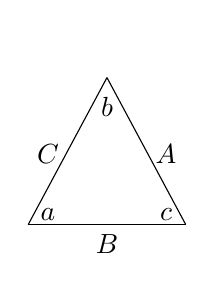
\begin{tikzpicture}[inner sep=0pt,minimum size=0mm]

\node () at (0,2.5) {};

\draw[] (0,0) -- (2,0);
\draw[] (0,0) -- (1,1.866);
\draw[] (2,0) -- (1,1.866);

\node () at (0.25,0.125){$a$};
\node () at (1.0,1.5) {$b$};
\node () at (1.75,0.125) {$c$};

\node () at (1.75,0.9){$A$};
\node () at (0.25,0.9) {$C$};
\node () at (1.0,-0.25) {$B$};

\end{tikzpicture}
\end{figure}
}

\begin{enumerate}

\item{\bf Given $a=b=c=60\degree$ and $A=1$, find $B$ and $C$.}\\

\tab \tab Using the law of sines:\\

\tab \tab $\frac{sin(a)}{A} = \frac{sin(b)}{B}$\\

\tab \tab $=\frac{sin(60\degree)}{1} = \frac{sin(60\degree)}{B}$\\

\tab \tab $\implies B = 1$\\

\tab \tab $\frac{sin(a)}{A} = \frac{sin(c)}{C}$\\

\tab \tab $=\frac{sin(60\degree)}{1} = \frac{sin(60\degree)}{C}$\\

\tab \tab $\implies C = 1$\\

\item{\bf Given $a=35\degree$, $b=55\degree$, and $C=2$, find $c$, $A$, and $B$.}\\

\tab \tab $a+b+c=180\degree$\\

\tab \tab $35\degree + 55\degree + c = 180\degree$\\

\tab \tab $\implies c = 90\degree$\\

\tab \tab Using the law of sines,\\

\tab \tab $\frac{sin(c)}{C} = \frac{sin(a)}{A}$\\

\tab \tab $\frac{sin(90\degree)}{2} = \frac{sin(35)}{A}$\\

\tab \tab $\frac{1}{2} = \frac{0.574}{A}$\\

\tab \tab $A = 1.147$\\

\tab \tab $\frac{sin(c)}{C} = \frac{sin(b)}{B}$\\

\tab \tab $\frac{sin(90\degree)}{2} = \frac{sin(55)}{B}$\\

\tab \tab $\frac{1}{2} = \frac{0.819}{B}$\\

\tab \tab $B =1.638$\\

\item{\bf Given $a=45\degree$, $B=2$, and $C=3$, find $A$, $b$, and $c$.}\\

\tab \tab Using the law of cosines,\\

\tab \tab $A^2 = B^2 + C^2 - 2BCcos(a)$\\

\tab \tab $A^2 = 2^2 + 3^2 -2(2)(3)cos(45\degree)$\\

\tab \tab $A^2 = 4 + 9 -12\frac{\sqrt(2)}{2}$\\

\tab \tab $A^2 = 13 - 6\sqrt{2}$\\

\tab \tab $A^2 = 13 - 6\sqrt{2}$\\

\tab \tab $A = \sqrt{13 - 6\sqrt{2}}$\\

\tab \tab $A = \sqrt{13 - 6\sqrt{2}}$\\

\tab \tab $A = 2.125$\\

\tab \tab Using the law of sines,\\

\tab \tab $\frac{sin(a)}{A} = \frac{sin(b)}{B}$\\

\tab \tab $\frac{sin(45\degree)}{2.125} = \frac{sin(b)}{2}$\\

\tab \tab $\frac{\frac{\sqrt{2}}{2}}{2.125} = \frac{sin(b)}{2}$\\

\tab \tab $sin(b) = \frac{\sqrt{2}}{2.125}$\\

\tab \tab $sin(b) = 0.665$\\

\tab \tab $b = asin(0.665) = 41.72\degree$\\

\tab \tab $\frac{sin(a)}{A} = \frac{sin(c)}{C}$\\

\tab \tab $\frac{sin(45\degree)}{2.125} = \frac{sin(c)}{3}$\\

\tab \tab $\frac{\frac{\sqrt{2}}{2}}{2.125} = \frac{sin(c)}{3}$\\

\tab \tab $sin(c) = 0.998$\\

\tab \tab $b = asin(0.998) = 93.23\degree$ Note: $sin(x) = sin(180\degree - x)$\\

\item{\bf Given $A=5$, $B=7$, $C=11$, find $a$, $b$, and $c$.}\\

\tab \tab Using the law of cosines,\\

\tab \tab $A^2 = B^2 + C^2 - 2BCcos(a)$\\

\tab \tab $25 = 49 + 121 - 154cos(a)$\\

\tab \tab $cos(a) = \frac{49 + 121 -25}{154}$\\

\tab \tab $cos(a) = \frac{145}{154}$\\

\tab \tab $a = acos(0.9416)$\\

\tab \tab $a = 19.7\degree$\\

\tab \tab $B^2 = A^2 + C^2 - 2ACcos(b)$\\

\end{enumerate}

\clearpage
\subsection{Chapter 11}

\begin{enumerate}

\item{\bf Convert these complex numbers to polar form: \\ $1,\  i ,\  -1,\  -i,\  1+i,\  i-1,\  -i-1,\  1-i,\  2+i,\  2+2i$}\\

\tab \tab $1 = 1\angle0\degree$\\

\tab \tab $i = 1\angle90\degree$\\

\tab \tab $-1 = 1\angle180\degree$\\

\tab \tab $-i = 1\angle270\degree$\\

\tab \tab $1+i = \frac{\sqrt{2}}{2}\angle45\degree$\\

\tab \tab $i-1 = \frac{\sqrt{2}}{2}\angle135\degree$\\

\tab \tab $-1-i = \frac{\sqrt{2}}{2}\angle225\degree$\\

\tab \tab $1-i = \frac{\sqrt{2}}{2}\angle315\degree$\\

\tab \tab $2+i = \sqrt{5}\angle26.57\degree$\\

\tab \tab $2+i = \sqrt{2}\angle45\degree$\\

\item{\bf Convert these complex numbers to rectangular form: \\ $1\angle0,\   1\angle90\degree,\  2\angle\frac{\pi}{6}\rad,\   3\angle-60\degree,\  1\angle\pi\rad,\  -2\angle\frac{\pi}{4},\  0\angle90\degree,\  0\angle20\degree$}\\

\tab \tab $1\angle0 = 1$\\

\tab \tab $1\angle90 = i$\\

\tab \tab $2\angle\frac{\pi}{6}\rad = \sqrt{3} + i$\\

\tab \tab $3\angle-60\degree = \frac{3/2} - i\frac{3\sqrt{3}}{2}$\\

\tab \tab $1\angle\pi\rad = -1$\\

\tab \tab $-2\angle\frac{\pi}{4} = -\sqrt{2} - i\sqrt{2}$\\

\tab \tab $0\angle90\degree = 0$\\

\tab \tab $0\angle20\degree = 0$\\

\item{\bf Simplify the following: \\ $(1+i)+(2+2i),\ (3+3i)-(1-i),\ (1\angle\frac{3\pi}{4}\rad)-i,\  (1\angle45\degree)+(1\angle-45\degree), $}\\

\tab \tab $(1+i)+(2+2i) = 3 + 3i$\\

\tab \tab $(3+3i)-(1-i) = 2 + 4i$\\

\tab \tab $(1\angle\frac{3\pi}{4}\rad)-i = -\frac{\sqrt{2}}{2} + \frac{\sqrt{2}-2}{2}i$\\

\tab \tab $(1\angle45\degree)+(1\angle-45\degree) = \sqrt{2}$\\

\item{\bf Simplify the following: \\ $(1+i)(1-i),\ (2+i)(3+3i),\ (1+i)(1\angle\frac{\pi}{4}\rad),\ (2\angle135\degree)(2\angle210\degree)$}\\

\tab \tab $(1+i)(1-i) = 2$\\

\tab \tab $(2+i)(3+3i) = 3 + 9i$\\

\tab \tab $(1+i)(1\angle\frac{\pi}{4}\rad) = \frac{2+\sqrt{2}}{2} + \frac{2+\sqrt{2}}{2}i$\\

\tab \tab $(2\angle135\degree)(2\angle210\degree) = 4\angle345\degree$\\

\item{\bf Simplify the following: \\ $\frac{1+i}{1-i},\ \frac{2+2i}{-3-i},\ \frac{1\angle\frac{\pi}{3}\rad}{1+i},\ \frac{1\angle30\degree}{1\angle-60\degree}$}\\

\tab \tab $\frac{1+i}{1-i} = i$\\

\tab \tab $\frac{2+2i}{-3-i} = \frac{-4-2i}{5}$\\

\tab \tab $\frac{1\angle\frac{\pi}{3}\rad}{1+i} = \frac{(\sqrt{3} + 1) + (\sqrt{3} - 1)i}{4}$\\

\tab \tab $\frac{1\angle30\degree}{1\angle-60\degree} = i$\\

\end{enumerate}

\clearpage
\subsection{Chapter 12}

\begin{enumerate}

\item{\bf What is Euler's formula?}

\tab \tab $e^{i\theta} = cos(\theta) + i sin(\theta)$\\

\item{\bf Use Euler's formula to derive the double-angle sine formula: \\ $sin(2\theta)=?$}

Starting with Euler's formula:\\

\tab \tab $e^{i\theta} = cos(\theta) + i sin(\theta)$\\

Using rearrangements from chapter 12,\\

\tab \tab $sin(\theta) = \frac{1}{2i}(e^{i\theta} - e^{-i\theta})$ \  and \  $cos(\theta) = \frac{1}{2}(e^{i\theta} + e^{-i\theta})$\\

So,\\

\tab \tab $sin(2\theta) = \frac{1}{2i}(e^{i2\theta} - e^{-i2\theta})$\\

\tab \tab $\implies sin(2\theta) = \frac{1}{2i}((e^{i\theta})^{2} - (e^{-i\theta})^{2})$\\

\tab \tab $\implies sin(2\theta) = \frac{1}{2i} (e^{i\theta} - e^{-i\theta}) (e^{i\theta} + e^{-i\theta}) $\\

\tab \tab $\implies sin(2\theta) = (sin(\theta))(2cos(\theta))$\\

\tab \tab $\implies sin(2\theta) = 2sin(\theta)cos(\theta)$\\

\item{\bf Use Euler's formula to find the phase offset between sine and cosine: \\ $sin(\theta + x) = cos(\theta) \implies ?$}

Starting with Euler's formula:\\

\tab \tab $e^{i\theta} = cos(\theta) + i sin(\theta)$\\

We are looking for $x$ such that $sin(\theta + x) = cos(\theta)$\\

So, \\

\tab \tab $sin(\theta + x) = cos(\theta)$\\

\tab \tab $\implies \frac{1}{2i}(e^{i(\theta + x)} - e^{-i(\theta + x)})= \frac{1}{2}(e^{i\theta} + e^{-i\theta})$\\

\tab \tab $\implies (e^{i(\theta + x)} - e^{-i(\theta + x)})= i(e^{i\theta} + e^{-i\theta})$\\

\tab \tab $\implies (e^{i\theta}e^{ix} - e^{-i\theta}e^{-ix})= ie^{i\theta} + ie^{-i\theta}$\\

\tab \tab $\implies e^{ix} = i$ \ and \ $-e^{-ix} = i$\\

\tab \tab $\implies e^{ix} = i$ \ and \ $\frac{1}{e^{ix}} = -i$\\

\tab \tab $\implies e^{ix} = i$ \ and \ $e^{ix} = -\frac{1}{i}$\\

\tab \tab $\implies e^{ix} = i$ \ and \ $e^{ix} = i$\\

\tab \tab $\implies cos(x) + isin(x) = i$\\

\tab \tab $\implies x = 90\degree$\\

\end{enumerate}
